%   Filename    : chapter_4.tex 
\section*{Chapter 3}
\section{Research Methodology}
This chapter lists and discusses the specific steps and activities carried out to complete the project. 

\subsection{Research Activities}

As illustrated in Figure \ref{fig:process diagram}, the researchers conducted a series of research activities. They have first consulted domain experts to gather data, clarify its interpretation, and discuss enhancements on the ontology’s structure. The gathered data was then encoded into the digital ontology, incorporating the suggested enhancements. Parallel to this, chatbot development  began, using only some of the initially encoded data to expedite progress rather than waiting for the completion of encoding all gathered folk narratives. The chatbot was trained and tested on the basis of specified metrics, then deployed on a website.

\begin{figure}[H]
    \centering
    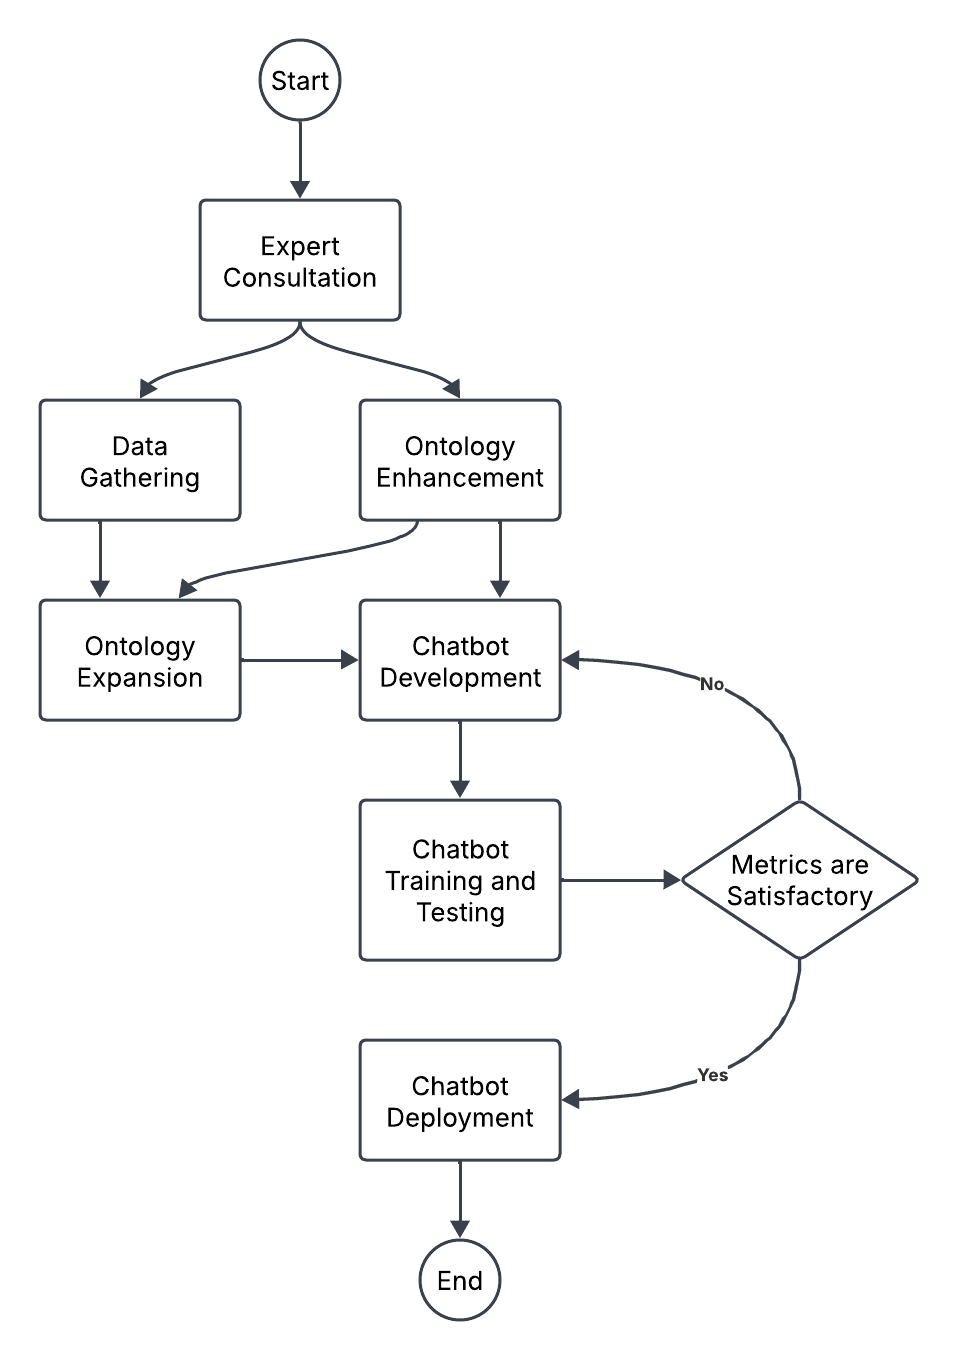
\includegraphics[width=0.8\linewidth]{figures/Process Diagram of Special Project.png}
    \caption{Process Diagram of Special Project}
    \label{fig:process diagram}
\end{figure}

\subsection{Ontology Development}
\subsubsection{Data Collection} 
    The researchers gathered Panayanon myths and legends from the terminal report by \citeA{dimzonmyths}, which compiles various aspects of West Visayan culture and was presented to the U.P. Visayas Center for West Visayan Studies (CWVS), a research and extension arm of UPV. In addition to this report, the researchers were provided with the accompanying digital ontology, which serves as the foundational groundwork for this special project. 
    
    Given the scope of the project, only stories from Panay Island were included and others were ignored. While the researchers considered incorporating additional stories from other sources, Mrs. Dimzon explained that research and anthologies from different sources might introduce classifications that differ from those used in her work. The researchers thought this may potentially overcomplicate the structure of the digital ontology; hence, they opted to work exclusively with her work.
    
\subsubsection{Ontology Enhancement} 
    Based on consultations with the domain expert Mrs. Dimzon, a few classes were created in the digital ontology. The new classes were created using Protégé, an open-source ontology editor that supports OWL (Web Ontology Language) for formalizing domain knowledge. Protégé has features such as logical constraints and reasoning, which were utilized in ensuring consistency and inferring class hierarchy. Each class was connected through relationships with other entities to create a structured and interconnected narrative representation. These additions enable the ontology to store more information, allowing users to apply specific filters when making more complex queries.

\subsubsection{Ontology Expansion}
    The researchers have consulted with Mrs. Dimzon in how to properly identify key story elements, and the contextual relationships between entities in a story. With this, the researchers closely read and examined each story from the collected data, looking for relevant story elements and relationships. From their findings, they expanded the digital ontology by populating it with new stories, entities, and relationships based on the enhanced ontological structure. 
    
    Protégé was utilized for ontology expansion for its extensive support in OWL files and SPARQL querying, reasoning, and consistency checking features.

\subsection{Chatbot Development}
\subsubsection{Chatbot Development Tools}
    The researchers developed a chatbot prototype that can handle English queries from users, query the ontology to search for relevant data, and present the information to the user in comprehensible English sentences. Specifically, the researchers utilized Python as the primary programming language to develop the chatbot, spaCy as the natural language processing (NLP) library to analyze and process user queries, Rasa as the machine learning framework to extract the entities and intents of user inputs, GraphDB as the knowledge base to host the ontology, and a natural language generation (NLG) server to generate conversational responses to the user.

\subsubsection{User Experience}
    To enhance user experience, the chatbot was designed to exhibit a conversational tone while maintaining the accuracy and professionalism required for ontology-based information retrieval. By incorporating NLG techniques, the chatbot aims to engage users with dynamic and contextually appropriate responses that emulate human-like interaction. This conversational approach is expected to improve user engagement and satisfaction, especially when addressing more complex queries that may require clarification or follow-up interactions.

    With this chatbot, users will be able to interact with the ontology in natural language in a conversational and friendly manner. This is in pursuit of data querying, which is \citeA{manansala2007}) third and final pillar of ontology frameworks. 

\subsubsection{Rasa Framework}
    Figure \ref{fig:rasa framework} shows the flow of data from user input to chatbot response generation. The ontology is converted into a graph database that can be queried for relevant information. The Rasa Agent works as a controller to easily orchestrate the dialogue flow of the chatbot, and manage the interaction of the different components. 
    
    When the user inputs a message, the NLU pipeline will first process it to extract its entities and intents. The extracted information is then passed through the Rasa Agent to the Dialogue Policies, which determine the appropriate action. If an external query is required, the Action Server requests information from the Knowledge Base. The data retrieved from the query are passed through an NLG server that contains Rasa's contextual response rephraser to generate more natural and conversational responses. The Rasa Agent receives this to then output the response to the user. The Tracker Store also receives the extracted entities, intents, and executed actions in order to maintain conversation history, which will help the Dialogue Policies make more context-aware decisions over time.

\begin{figure}[H]
    \centering
    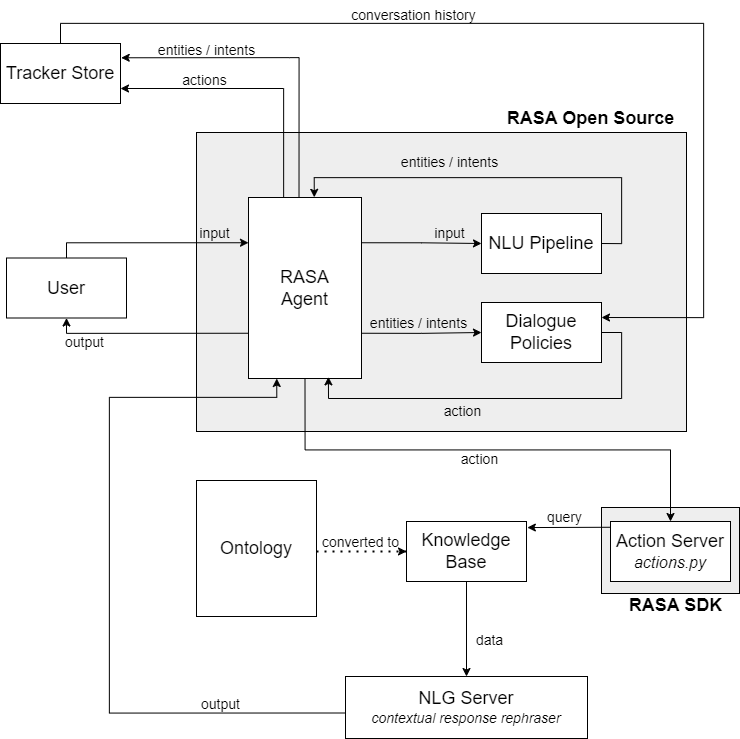
\includegraphics[width=\linewidth]{figures/Rasa Framework.png}
    \caption{Diagram of Rasa Framework}
    \label{fig:rasa framework}
\end{figure}

    Figure \ref{fig:nlu pipeline} illustrates Rasa's natural language understanding pipeline. The first component is the spaCy tokeniser, which splits the user's input into tokens. The second component is the spaCy featurizer, which is a dense featurizer that extracts features used for entity extraction, intent identification of the user's message, and response classification. The regex featurizer is a sparse featurizer that creates a vector representation of the user's message using regular expressions for the purpose of entity extraction and intent identification. Next is the lexical syntactic featurizer, which is a sparse featurizer that creates lexical and syntactic features for a user's message for the purpose of entity extraction. The fifth component is the count vectors featurizer, which generates a bag-of-words representation of the bot user's message, intent, and response for the purpose of intent identification and response selection. The DIET Classifier is a multi-task transformer architecture that is responsible for intent classification and entity extraction. The final component is the Entity Synonym Mapper that maps entities to their synonyms if they appeared in the training data. The extracted entities and identified intents in the NLU pipeline will then be passed to the chatbot dialogue policies to determine the appropriate actions that the bot will perform. 

    The components within the pipeline are used to process the user's input and extracts entities and intents from the user's input. This will be then queried through the knowledge base. Finally, the query results will be formatted in English using NLP techniques. 

\begin{figure}[H]
    \centering
    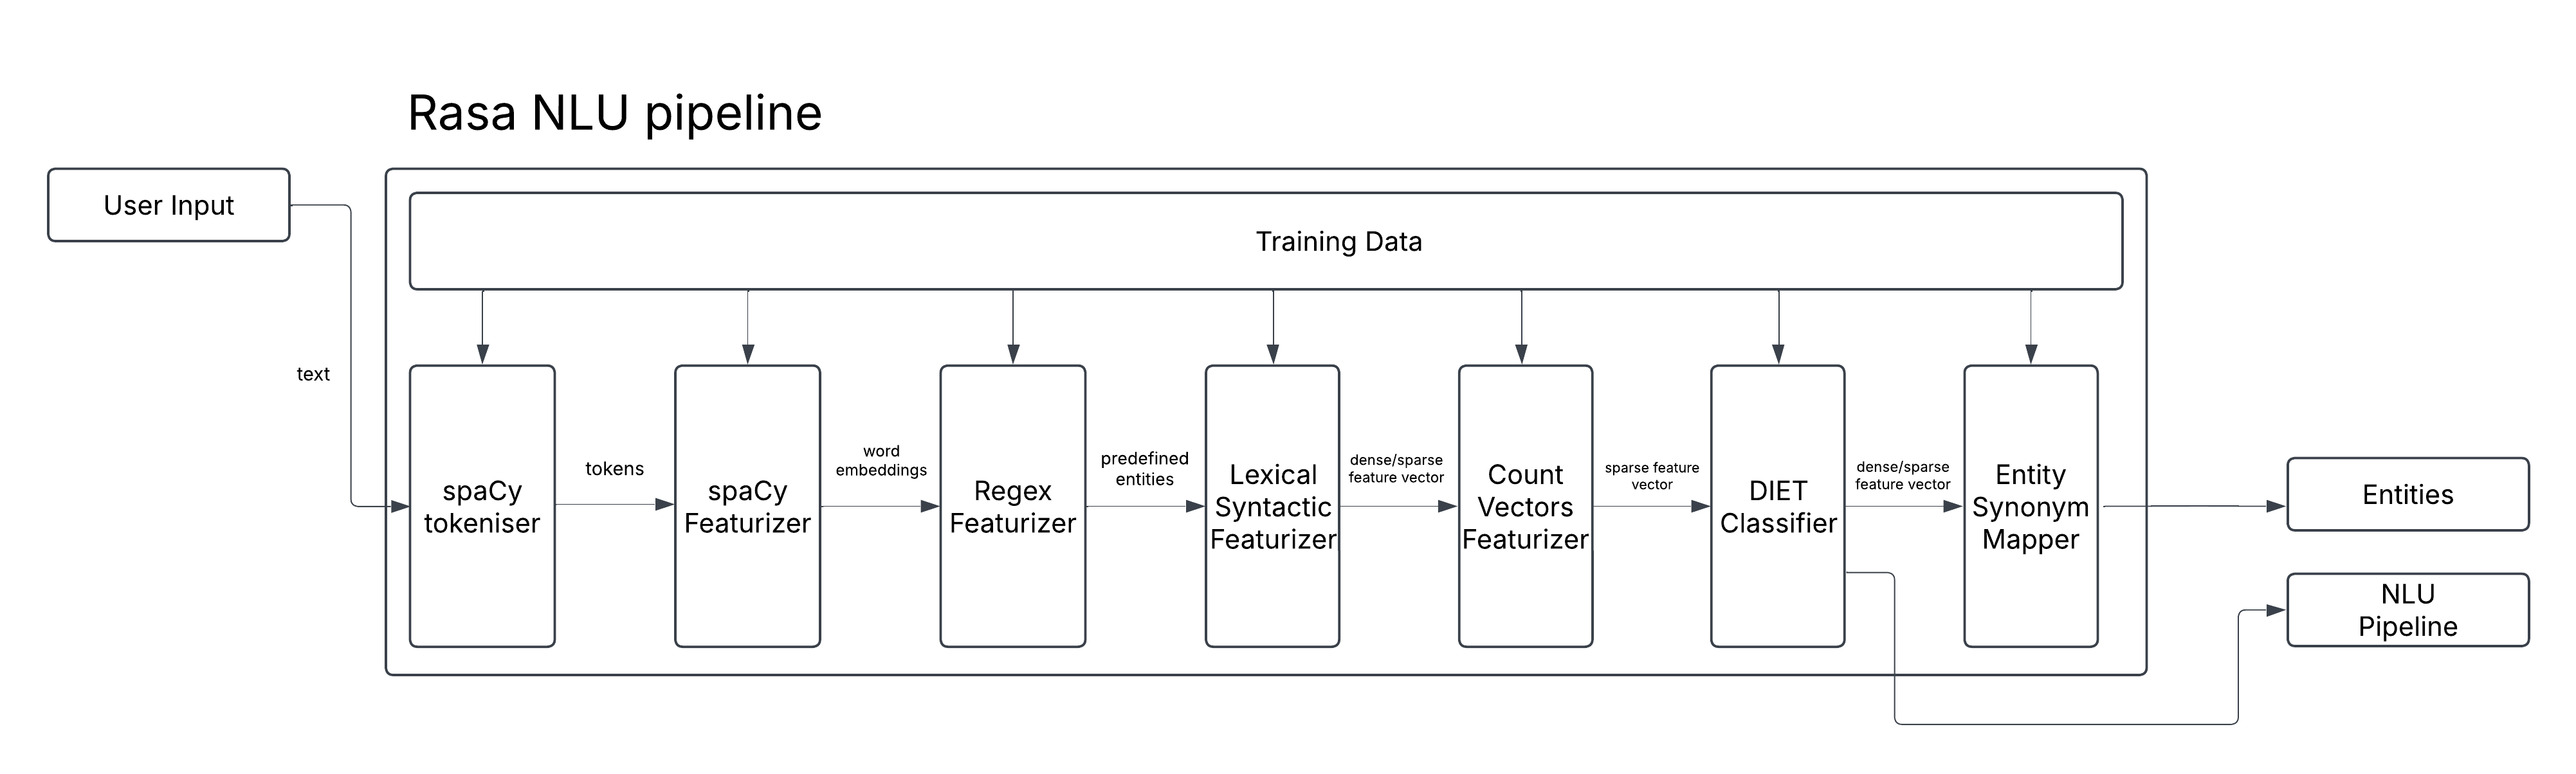
\includegraphics[width=\linewidth]{figures/NLU Pipeline.png}
    \caption{Diagram of NLU Pipeline}
    \label{fig:nlu pipeline}
\end{figure}

\subsubsection{Chatbot Testing}
    The evaluation of the PAROT model by Ochieng (2020) involved the use of QALD-9 challenge metrics, including accuracy, recall, and F-measure. Similarly, the utilization of these metrics will be applied in the evaluation of the model under development of this special project.

    With each iteration of the chatbot, the researchers will perform tests to verify chatbot query accuracy and response relevance, assess user interaction with the chatbot, and measure response times and optimize as needed.
    
\subsection{System Deployment}
\subsubsection{Rasa Chatbot}
    The chatbot, developed using the Rasa framework, was deployed via the Google Kubernetes Engine (GKE), a managed Kubernetes service provided by the Google Cloud Platform (GCP). The use of GKE facilitated the creation of Kubernetes clusters without the manual setup of the Kubernetes infrastructure \cite{sullivan2023}. The deployment process followed the guidelines outlined in the Rasa Open Source documentation.

% [Rasa Docs, https://legacy-docs-oss.rasa.com/docs/rasa/deploy/deploy-rasa/]

\subsubsection{PanayHub Website}
    Website hosting was facilitated through the Render.com platform, selected for its usability and streamlined deployment capabilities. Render.com provides infrastructure for hosting websites and servers, with integrated support for popular Git repository hosting services such as GitHub and GitLab. This integration enables automated deployment triggered by each new commit, enhancing development workflow efficiency.

    Figures \ref{fig:panayhub-home}, \ref{fig:panayhub-contact}, and \ref{fig:panayhub-chatbot} present the user interface of the website. Figure \ref{fig:panayhub-home} illustrates the homepage, which functions as the primary landing page and navigation hub for users. Figure \ref{fig:panayhub-contact} depicts the \textit{Contact Us} page, which provides users with a channel for communication with researchers and affiliated institutions. Lastly, Figure \ref{fig:panayhub-chatbot} displays the chatbot interface, allowing user interaction with the chatbot for inquiries related to the folk narratives of Panay.

    \begin{figure}
        \centering
        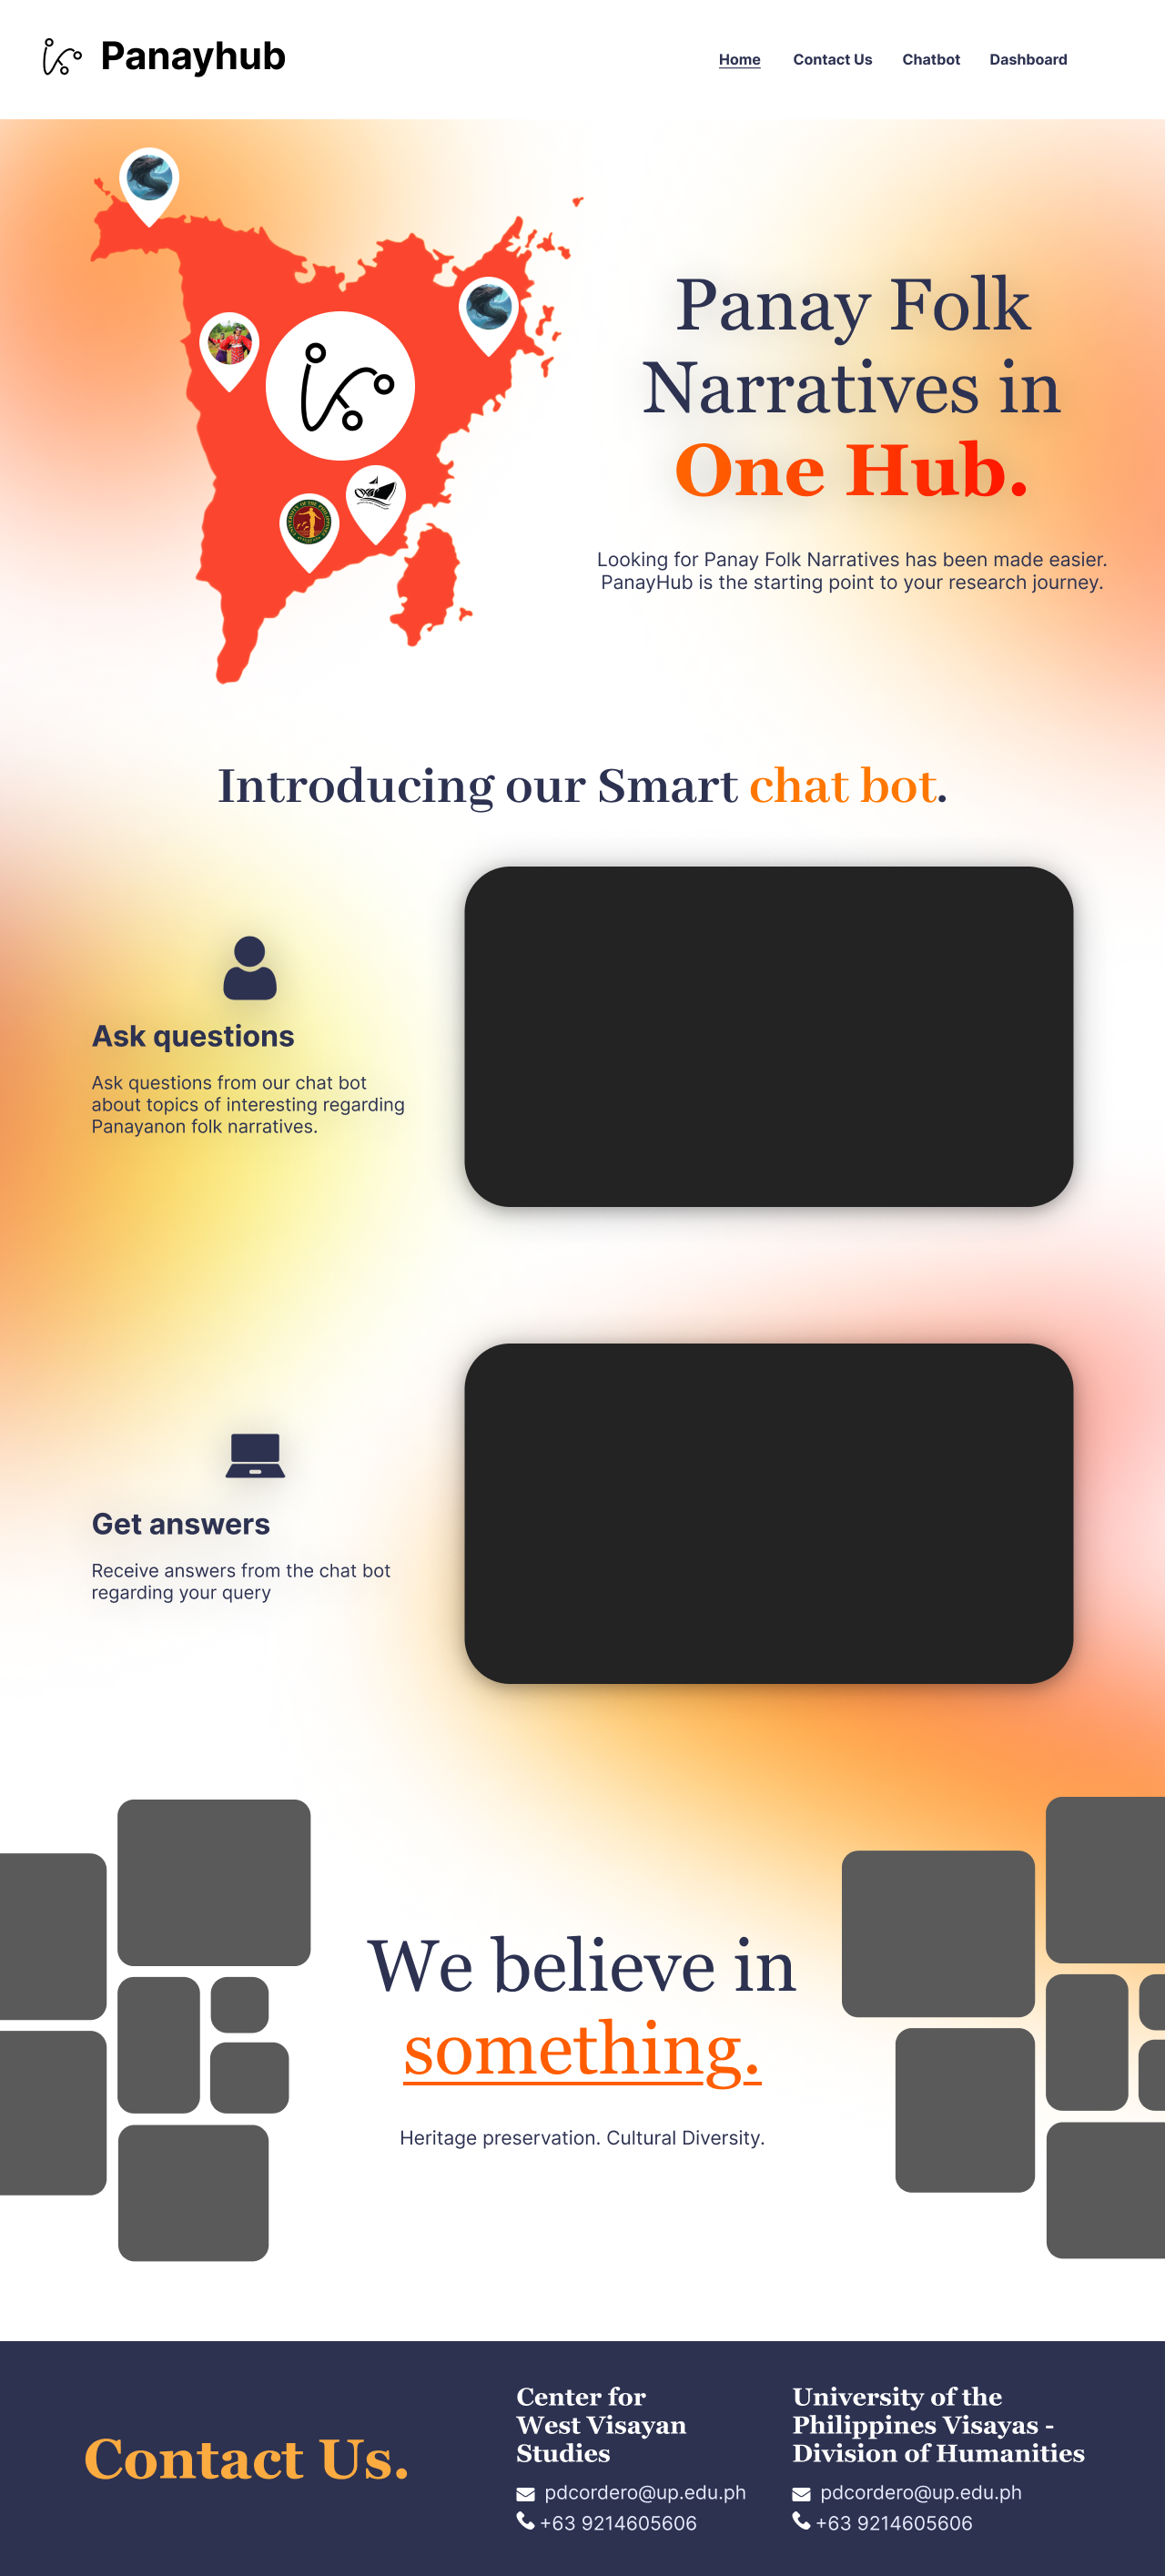
\includegraphics[width=0.5\linewidth]{figures/Home.png}
        \caption{Homepage of PanayHub}
        \label{fig:panayhub-home}
    \end{figure}
    
    \begin{figure}
        \centering
        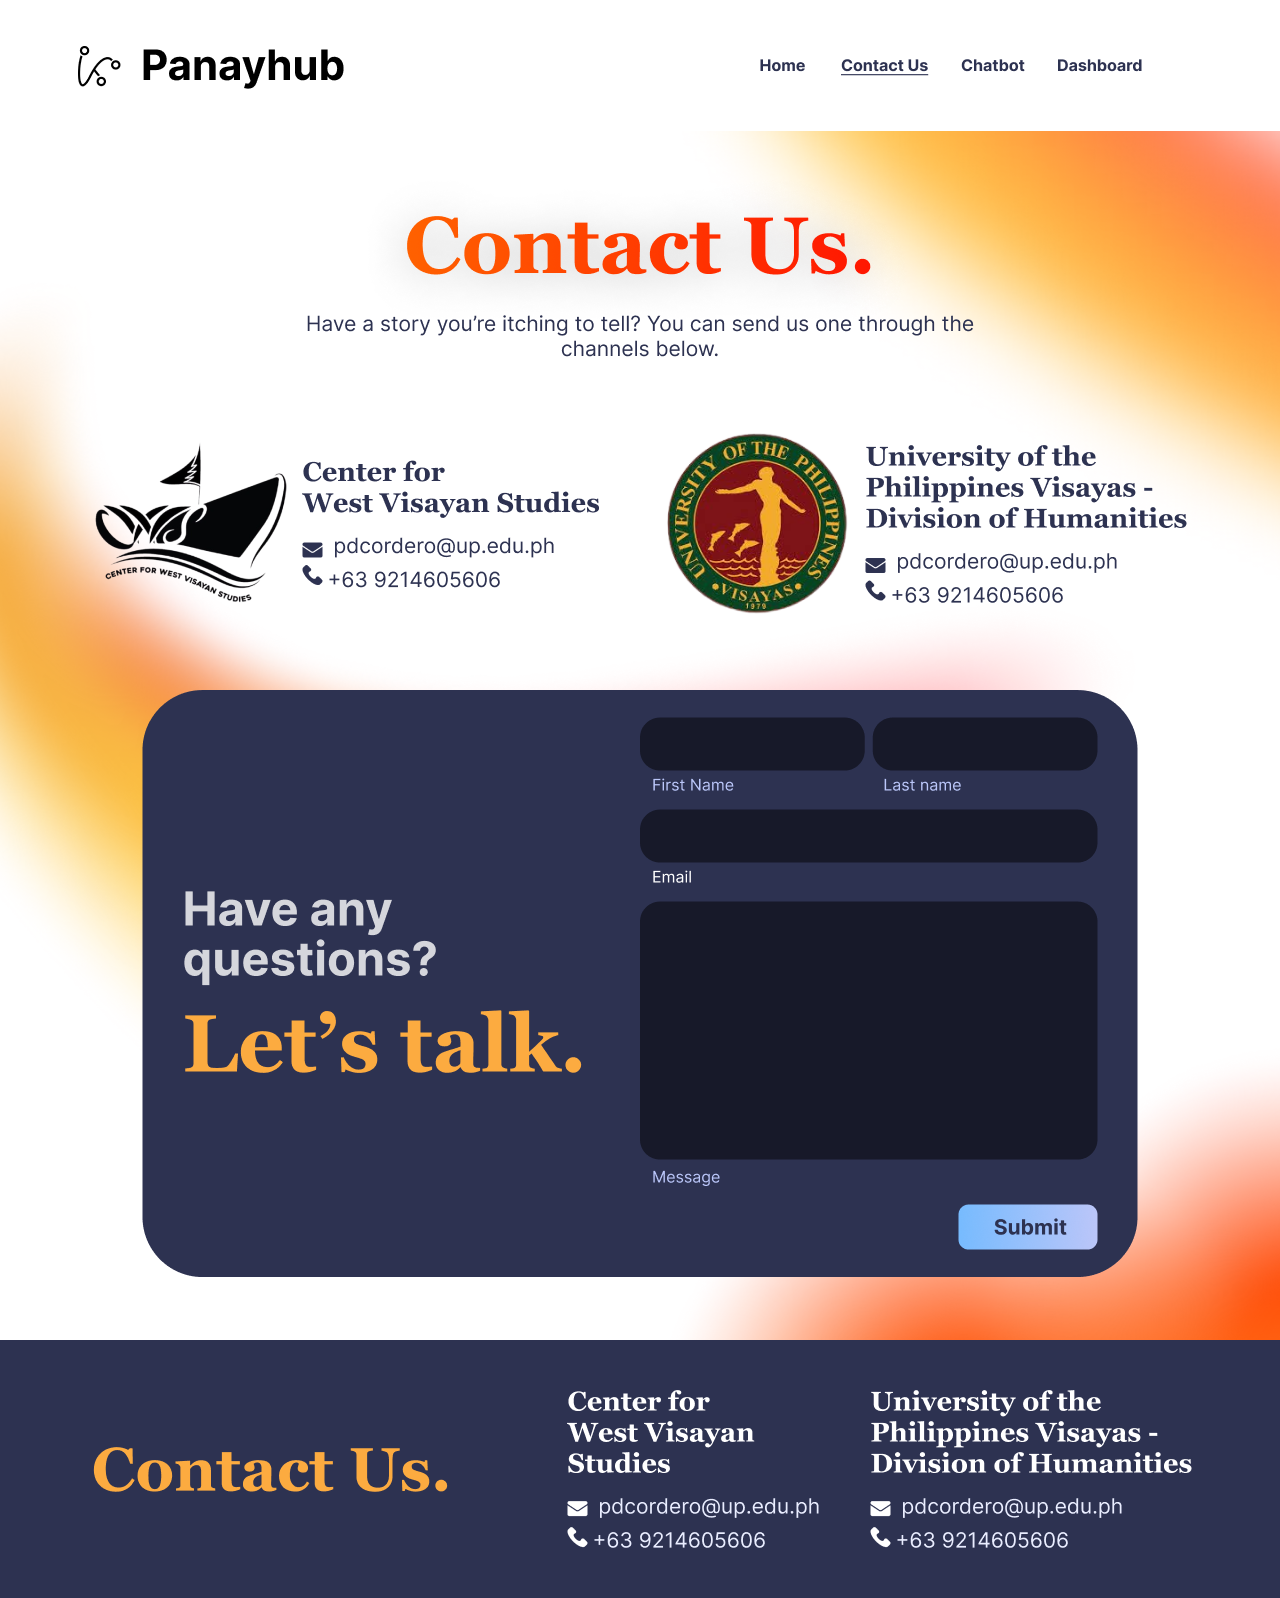
\includegraphics[width=0.5\linewidth]{figures/Contact Us.png}
        \caption{Contact Us page of PanayHub}
        \label{fig:panayhub-contact}
    \end{figure}

    \begin{figure}
        \centering
        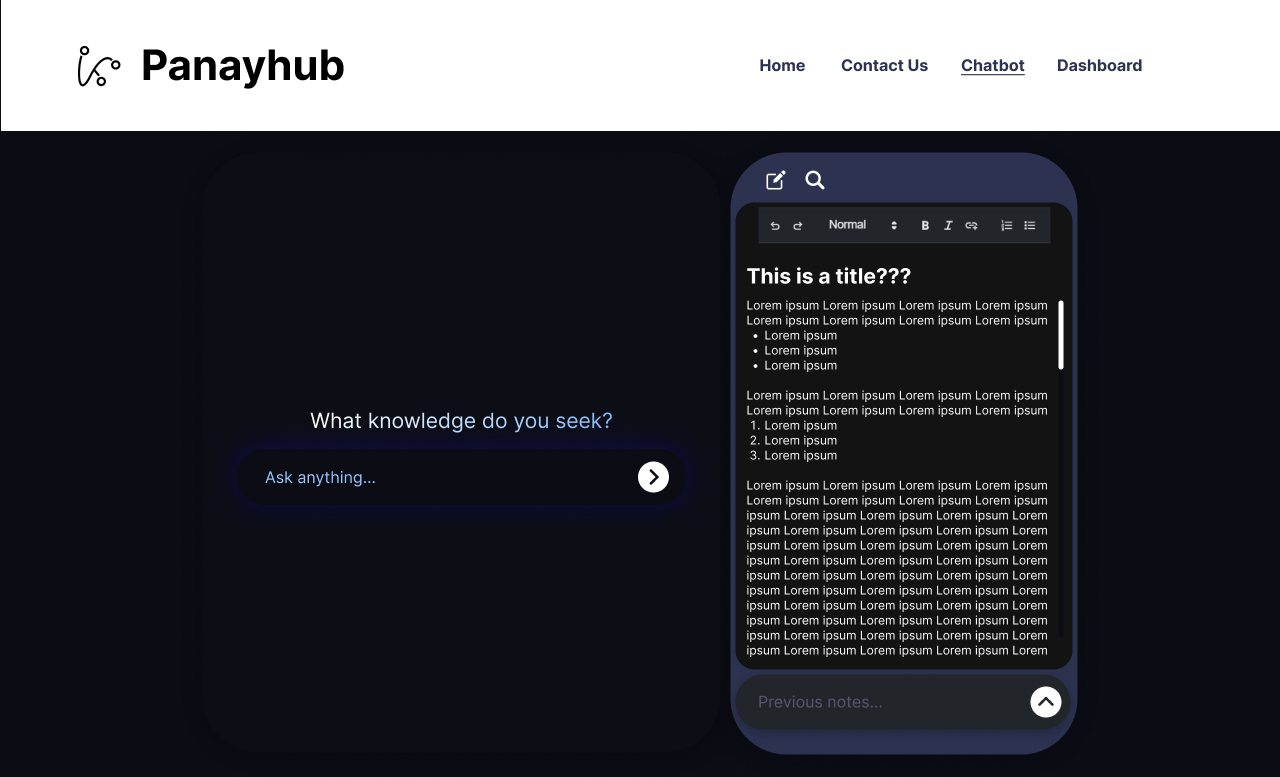
\includegraphics[width=0.5\linewidth]{figures/Chatbot.png}
        \caption{Chatbot page of PanayHub}
        \label{fig:panayhub-chatbot}
    \end{figure}